\documentclass[final]{beamer}
\mode<presentation>
{
 % \usetheme{collis} 
\usetheme{ANLARM}
}
\graphicspath{{figures/}}

\usepackage{times}
\usepackage{amsmath,amssymb}
\usepackage[english]{babel}
\usepackage[latin1]{inputenc}
\usepackage[printwatermark]{xwatermark}
\usepackage[orientation=landscape,size=a0]{beamerposter}  % e.g. custom size poster
\usepackage{tikz}
\addtobeamertemplate{block begin}{\pgfsetfillopacity{0.8}}{\pgfsetfillopacity{1}}


\usebackgroundtemplate{
\tikz\node[opacity=0.5] {\includegraphics[height=\paperheight,width=\paperwidth]{figures/radar2.png}};}


\title{\huge Architectures for Rainfall Property Estimation From Polarimetric Radar}
\author[Collis et al.]{Scott Collis\textsuperscript{1} {\texttt{scollis@anl.gov}},
 Scott Giangrande\textsuperscript{2},
  Jonathan Helmus\textsuperscript{1}
   and Silke Troemel\textsuperscript{3}}
\institute[Argonne]{
1: Argonne National Laboratory Argonne, IL United States \\
2: Brookhaven National Laboratory, Upton, NY United States\\
3: Meteorologisches Institut der Universit{\"a}t Bonn, Bonn, Germany}
\date{\today}
\begin{document}
\begin{frame}{} 
 \begin{columns}[t]
    \begin{column}{.3\linewidth}
  \vfill
  %%%%%%%%%%%Intro Block %%%%%%%%%%%%%%%%%%%%%%%%
      \begin{block}{Introducton}
        \begin{columns}[t]
          \begin{column}{.6\linewidth}
          %%%%%%%%%%%%%%%Col 1: Text%%%%%%%%%%%%%%%%%%%%
        \begin{itemize}
        \item The Department of Energy's ARM Climate Research Facility operates a network of 5 and 3 cm scanning radar systems.
        \item Fixed sites are at the Azores, Southern Great Plains of Oklahoma and the town of Barrow on the North Slope of Alaska                                
         \end{itemize}
         \end{column}
          \begin{column}{.4\linewidth}
          %%%%%%%%%%%%%%%%Col 2: Figure%%%%%%%%%%%%%%%%%%%
           \vskip0ex
            \centering    
           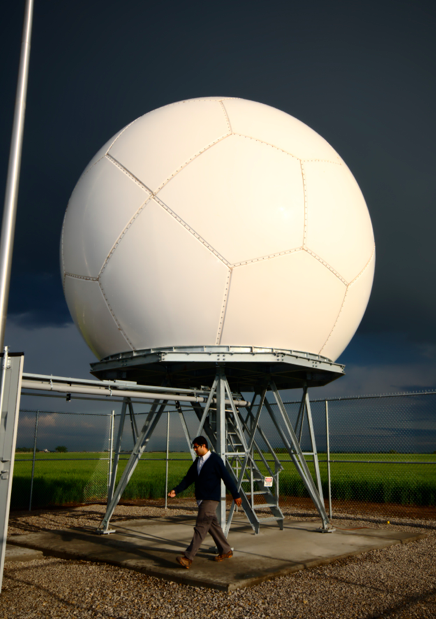
\includegraphics[width=0.7\linewidth]{figures/csapr.png}\\[1ex]            
          \end{column}
         \end{columns}
         \end{block}
         
         
        \begin{block}{The \textcolor{red}{Py}thon \textcolor{red}{A}RM \textcolor{red}{R}adar \textcolor{red}{T}oolkit}
                \begin{columns}[t]
                    \begin{column}{.6\linewidth}
                        \begin{itemize}
                            \item Working with radar data to generate geophysical products follows a similar basic path irrespective of what insight is sought:
			   \item Read in the data
                            \item  Correct the data in radar coordinates
                            \item  Map the data to a model like grid
                            \item  Use models of interaction to retrieve atmospheric parameters from remotely sensed quantities
                            \item  Using the Python language and community based software tools like Scientific 
                            Python our team has developed an open source community tool for interacting with radar data. 
                            \item  This is an open-source (BSD) licensed Argonne invention.
                       \end{itemize}
                   \end{column}
                   \begin{column}{.4\linewidth}
                   \vskip0ex
                       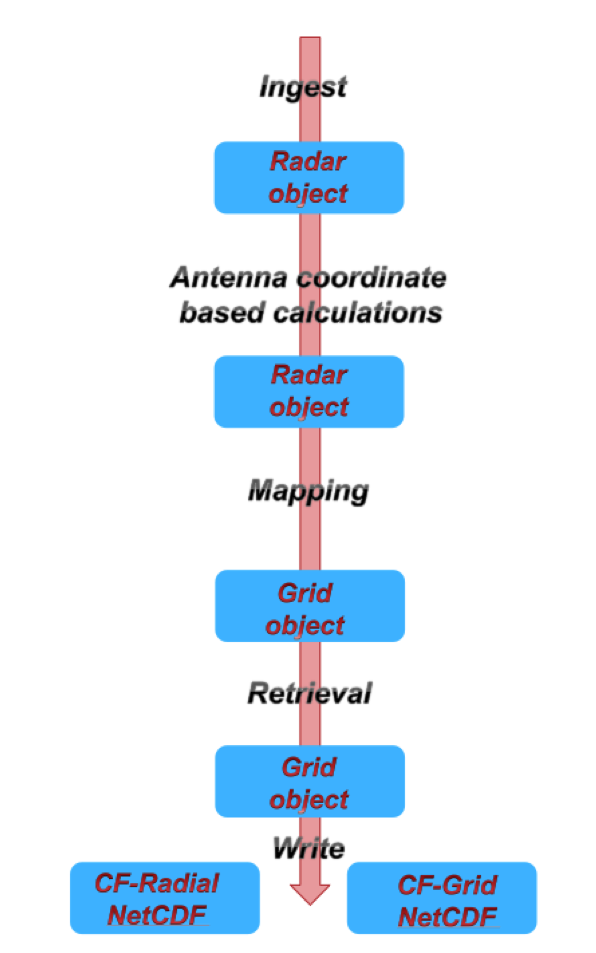
\includegraphics[width=0.9\linewidth]{figures/pyart-flow}\\[1ex]   
                   \end{column}
               \end{columns}
         \end{block}
         

     

    \end{column}
   %COL 2%
      \begin{column}{.3\linewidth}
  \vfill
 
     \begin{block}{Quantitative Precipitation Estimates}
 	\begin{columns}[t]
		\begin{column}{.4\linewidth}
		\end{column}
                \begin{column}{.6\linewidth}
           		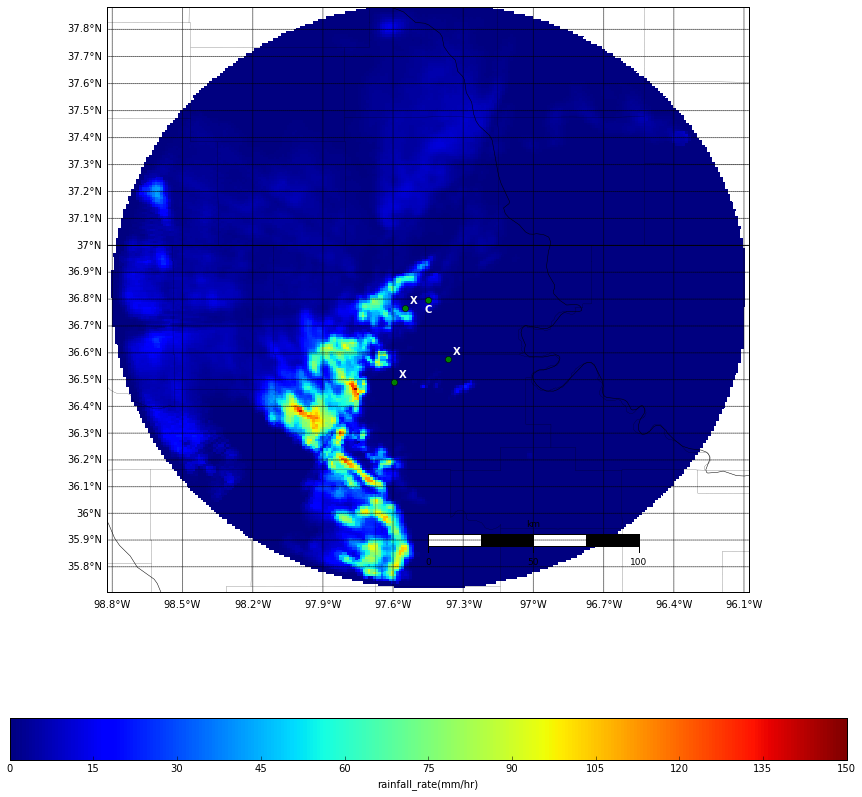
\includegraphics[width=1.0\linewidth]{figures/qpe.png}\\[1ex]     
 		\end{column}
	\end{columns}
      \end{block}


    \end{column}
%COL 3%
  \begin{column}{.3\linewidth}
  \vfill
   \begin{block}{Advective interpolation}
 	\begin{columns}[t]
		\begin{column}{.4\linewidth}
		\end{column}
                \begin{column}{.6\linewidth}
           		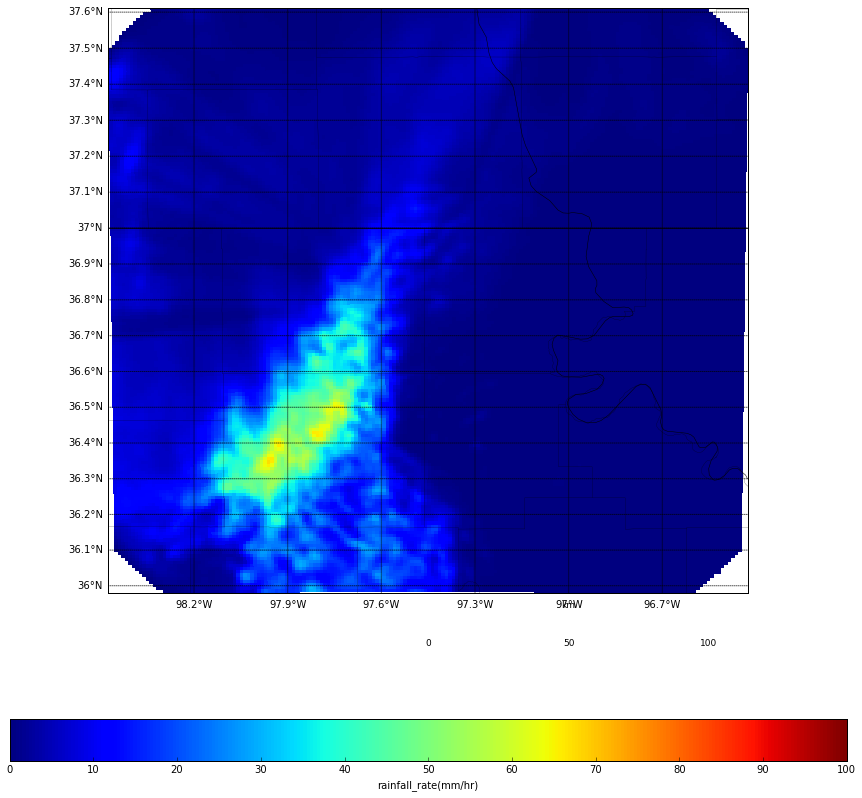
\includegraphics[width=1.0\linewidth]{figures/basic_accumulation.png}\\[1ex]     
            		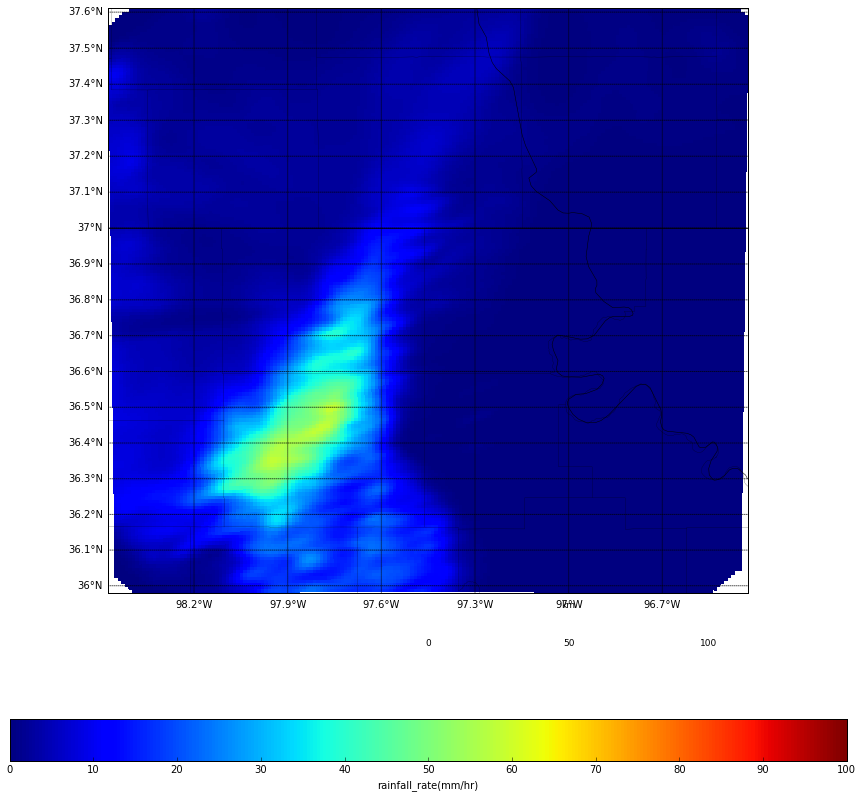
\includegraphics[width=1.0\linewidth]{figures/advective_accum.png}\\[1ex]  
 		\end{column}
	\end{columns}
      \end{block}
   
   
 
      \begin{block}{Introduction}
        \begin{itemize}
        \item automatic sign language recognition system                                    %what
        \item \alert{necessary for communication} between deaf and
          hearing people
        \item \alert{continuous} sign language recognition,
          \alert{several} speakers, \alert{vision-based} approach, \alert{no
            special hardware}
        \item large vocabulary speech recognition (LVSR) system to
          obtain a textual representation of the signed
          sentences 
        \item evaluation of speech recognition techniques on \alert{publicly
          available sign language
          corpus}
        \end{itemize}
      \end{block}

    \end{column}

  \end{columns}


  \vfill
\end{frame}
\end{document}


%%%%%%%%%%%%%%%%%%%%%%%%%%%%%%%%%%%%%%%%%%%%%%%%%%%%%%%%%%%%%%%%%%%%%%%%%%%%%%%%%%%%%%%%%%%%%%%%%%%%
%%% Local Variables: 
%%% mode: latex
%%% TeX-PDF-mode: t